\chapter{Development}
The goal of this chapter is to illustrate the new implementations and changes to the project's software, describing the previous features' improvements, the new ones and the way in which they have been achieved.
\bigbreak

In the previous project's code, some time and memory optimizations have been made, minor bugs have been found and fixed and some other improvements have been done (as replacing deprecated methods and libraries with newer ones).

\section{MQTT QoS2 caching}
As mentioned in the \textit{Unsolved Issues} chapter of Dario Piotrowicz's thesis \cite{Pio19}, there was a problem with unreliable Wi-Fi networks (an issue in the library's GitHub repository is still open \cite{githubQos2Issue}): all messages generated while a broken client-broker connection were not stored to be sent when the connection is re-established.\\
To solve that issue have been implemented two caching queues, one for each connection: the playing session one and the neural network's pattern collection one. The cache size has been set to a safe value of 32 kilobytes, the biggest value that is always free while the program running; bigger values led the Photon out of memory.
The maximum number of messages that can be cached is stored in the \texttt{cache\_size} variable. With a maximum message size of 512 characters (511 effective characters because of the null terminated string), the value is easily calculated as 32.

Follows the playing session's connection caching implementation; the neural network one is analogous.
\bigbreak

\begin{lstlisting}[style=CPPStyle]

	...

	// ready to send the data (publishString) to the client
	if (client.isConnected()) {
        while (cached_messages.size() > 0) {
			// send cached messages
            std::string msg = cached_messages.front();
            cached_messages.pop();
			client.publish("motiontracker/" + ID,
							msg.c_str(),
							MQTT::QOS2);
        }
		client.publish("motiontracker/" + ID,
						publishString,
						MQTT::QOS2);
    } else if (cached_messages.size() < cache_bound) {
		// save message in cache
        std::string msg(publishString);
        cached_messages.push(msg);
    }

	...

\end{lstlisting}
\bigbreak

This solution has made possible to damper temporary disconnections caused by instable connections.

\section{Motion capture}
In the software's previous version, developed and improved by Dario Piotrowicz \cite{Pio19} from the Marco Lanini's project \cite{Lan17}, the data processed by the device and sent to the server were:
\begin{itemize}
	\item yaw, pitch and roll angles;
	\item acceleration with components in spherical coordinates system;
	\item raw gyroscope data;
	\item a velocity approximation
\end{itemize}
and the data basically flowed like as shown in the following schema:

\begin{center}
	\begin{figure}[ht!]
		\makebox[\textwidth]{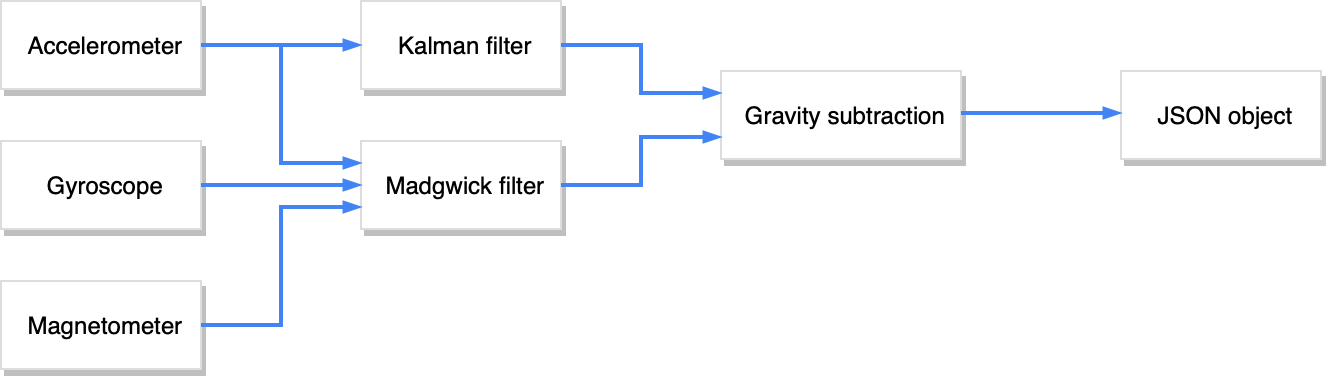
\includegraphics[width=0.65\paperwidth]{img/data_fusion_old.png}}
		\caption{Previous data fusion schema.}
	\end{figure}
\end{center}
\bigbreak

This work's aim was to detect \textit{discriminating features among different playing patterns}, by collecting and analyzing the sensors data stream; the analysis followed the flow in the data fusion schema, except for the velocity approximation.
\bigbreak

The velocity approximation, calculated by the \textit{Velocimeter} \cite{Pio19} was early excluded because of the practical difficulty in obtaining realistic values using only inertial sensors, where measurement errors are unavoidable, especially for miniature MEMS sensors. Direct integration of acceleration often causes unrealistic drifts in velocity, due to errors propagation; furthermore, measured acceleration not only carries random noise, but also presents with offset caused by temperature drift, resulting in estimation errors accumulated by integration process \cite{Du15, Est14, Kow15, Liu01, Sei07, UsingAcc, Woo07, Yan06}, that results in low accuracy. Were particularly problematic stillness detection after a movement (especially for that uniformly-like decelerated motion like the truck toy that stops by itself after a impulse from the back, where the velocity graph resulted in a peak toward zero instead of the real decrease), and repetitive light accelerations, like the one generated by the rolling of the tessellated tyres, that resulted in non-present velocities readings.

\begin{center}
	\begin{figure}[ht!]
		\makebox[\textwidth]{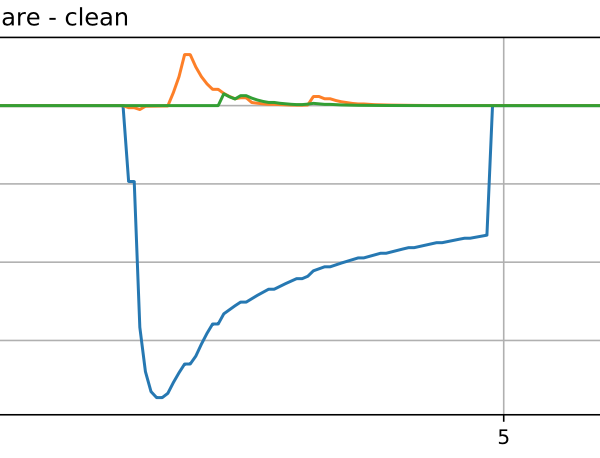
\includegraphics[width=0.2\paperwidth]{img/plots/square.png}}
		\caption{Square wave and non-present accelerations.}
	\end{figure}
\end{center}

The first analysis' phase dealt with raw accelerometer data, but the signal's noisiness and the presence of gravity have induced to desist. Nevertheless, more often than not the main waveform was recognizable, especially for movements with strong accelerations (that simply increase the signal-to-noise ratio).
\bigbreak

The analysis moved to Kalman-filtered data, which revealed much cleaner and smoother, but still included gravity; thus it would have been necessary a more complex training data collection, due to the lack of orientation invariance (the gravity decomposes among the axes in accordance with device's orientation, adding to other accelerations; in order to obtain such invariance it would be needed to collect every pattern with the device rotated in any possible angle).\\
Nevertheless, gravity-free acceleration data were computed by the device (with the help of Madgwick's fusion algorithm) and sent to the server but \textit{not stored in the database}, only used for the 3D visual representation, both in training and session recording phase. It was decided to keep such data and analyze it, to see whether it was reliable over time.
\bigbreak

Some testing showed quickly that there was an error in the yaw angle calculation: the more the device was moved, the more the yaw diverged (consequently the accelerations no longer matched the device's orientation). The error's cause was discovered to be the Madgwick's algorithm implementation, more precisely the lack of yaw's convergence in its error-correction gradient descent phase. Unfortunately, different algorithm implementations that included the correction, and different values of the algorithm's gain parameter (the magnitude $\beta$ of the gyroscope measurement error\footnote{Increasing $\beta$ leads to faster bias corrections and higher sensitiveness to lateral accelerations.} \cite[13]{Mad10}) have no given better results over time, and worse, sometimes ghost accelerations were found. The Lanini's version has been kept and the troubleshooting continued.
\bigbreak

The yaw's measurement was heavily affected by rotations around the Earth's $z$-axis (in other words, over the plane generated by the $x$ and $y$ axis), and the bigger the pitch angle, the bigger the error, as shown in the table below. Pitch and roll, on the contrary, were calculated without errors.
\bigbreak

\begin{table}[ht!]
	\centering
	\begin{tabular}{c|c c}
	\textbf{Pitch} ($^{\circ}$) & \textbf{Mean error} ($^{\circ}$) & \textbf{Standard deviation} ($^{\circ}$) \\ \hline
	0                           & -47.12                           & 0.94                                     \\
	20                          & -47.67                           & 1.88                                     \\
	40                          & -51.14                           & 1.45                                     \\
	60                          & -58.14                           & 1.73                                     \\
	80                          & -57.80                           & 0.75
	\end{tabular}
	\caption{Yaw errors after a 360$^{\circ}$ rotation with different pitch angles.}
\end{table}

Little yaw variations were noticed also with pitch-only movements: after a 360$^{\circ}$ rotation, the mean error was 0.47$^{\circ}$ with a standard deviation of 0.11$^{\circ}$.

\begin{center}
	\begin{figure}[ht!]
		\makebox[\textwidth]{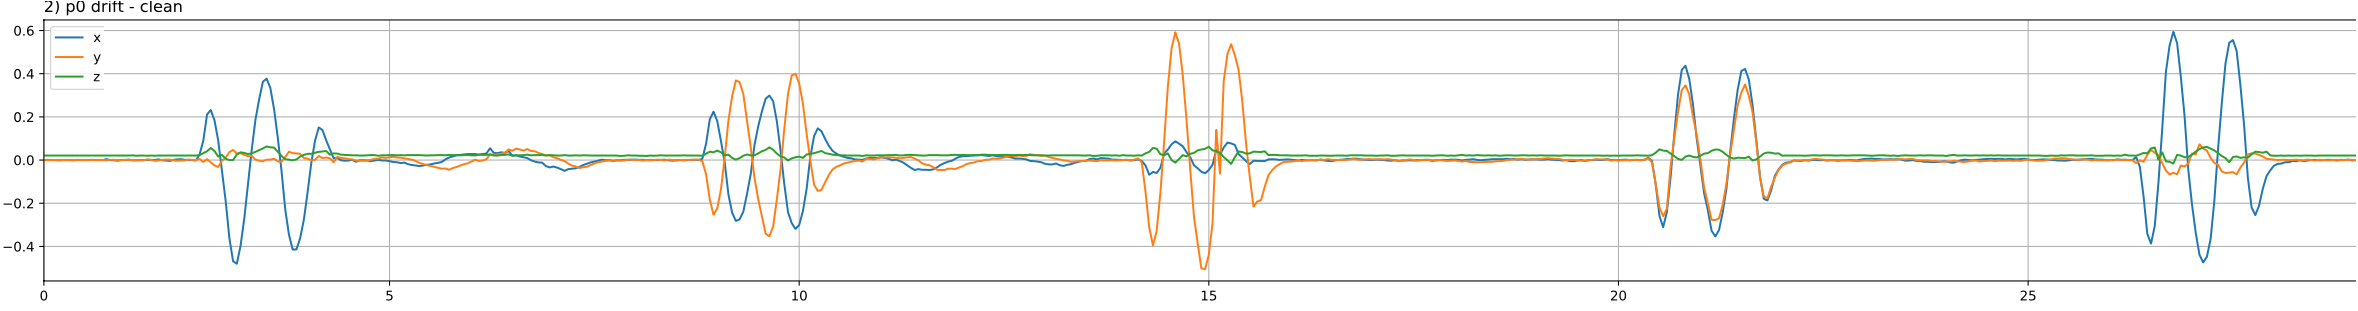
\includegraphics[width=0.6\paperwidth]{img/plots/drift.png}}
		\caption{Different accelerations for the same pattern.}
	\end{figure}
\end{center}

During some tests, it was noticed that recordings of the same pattern with different device orientations didn't split the acceleration differently among axes, revealing that the reference system was integral with the Earth's center instead of the device's sensor. To align it back, the acceleration vector has been rotated by the 3 angles (of \textit{yaw, pitch and roll}) given by the Madgwick's algorithm, and that, as shown below, solved both problems: the device orientation has been aligned with the accelerations, and the reference system was global.
\bigbreak

The rotation has been performed through a 3D rotation matrix. But what is a rotation matrix?\\
In two dimensions, a rotation matrix $R \in \mathbb R^{2 \times 2}$ is a matrix that is used to perform a rotation in Euclidean space. Given a vector $\vec u \in \mathbb R^2$ and an angle $\theta \in \mathbb R$, the vector $\vec u$ rotated through an angle $\theta$ can be written as $R(\theta) \vec u$.\\
The matrix

\[
	R =
	{\begin{pmatrix}
		\cos \theta & -\sin \theta \\
		\sin \theta & \cos \theta
	\end{pmatrix}}
\]
rotates points in the $xy$-plane counterclockwise in a \textit{right-handed coordinate system} ($y$ counterclockwise from $x$) through an angle $\theta$ with respect to the $x$ axis about the origin of a two-dimensional Cartesian coordinate system. To perform the rotation on a plane point with standard coordinates $\vec u$ = (x, y), it should be written as column vector, and multiplied by the matrix $R$ \cite{WikipediaRotationM}:
\bigbreak

\[
	R \vec u =
	{\begin{pmatrix}
		\cos \theta &-\sin \theta \\
		\sin \theta &\cos \theta
	\end{pmatrix}}
	\cdot
	{\begin{pmatrix}
		x \\
		y
	\end{pmatrix}} =
	{\begin{pmatrix}
		x\cos \theta -y\sin \theta \\
		x\sin \theta +y\cos \theta
	\end{pmatrix}}
\]
\bigbreak

How to represent \textit{yaw, pitch and roll}?
\bigbreak

A \textit{yaw} is a CCW rotation of $\alpha$ on the $z$-axis. The rotation matrix is
\[
	R_z(\alpha) =
	\begin{pmatrix}
		\cos\alpha & -\sin\alpha & 0 \\
		\sin\alpha & \cos\alpha & 0 \\
		0 & 0 & 1
	\end{pmatrix}
\]
Note that the upper left values compose a 2D rotation matrix, and the coordinates on the third dimension (around whom the rotation happens) are left unchanged. The same applies to the other two matrices, but with the second and the first dimension.
\bigbreak

A \textit{pitch} is a CCW rotation of $\beta$ on the $y$-axis. The rotation matrix is
\[
	R_y(\beta) =
	\begin{pmatrix}
		\cos\beta & 0 & \sin\beta \\
		0 & 1 & 0 \\
		-sin\beta & 0 & \cos\beta
	\end{pmatrix}
\]

A \textit{roll} is a CCW rotation of $\gamma$ on the $x$-axis. The rotation matrix is
\[
	R_x(\gamma) =
	\begin{pmatrix}
		1 & 0 & 0 \\
		0 & \cos\gamma & -\sin\gamma \\
		0 & sin\gamma & \cos\gamma
	\end{pmatrix}
\]
\begin{gather*}
	R(\alpha, \beta, \gamma) = R_z(\alpha) R_y(\beta) R_x(\gamma) = \\
	\begin{pmatrix}
		\cos\alpha \cos\beta & \cos\alpha \sin\beta \sin\gamma - \sin\alpha \cos\gamma & \cos\alpha \sin\beta \cos\gamma + \sin\alpha \sin\gamma \\
		\sin\alpha \cos\beta & \sin\alpha \sin\beta \sin\gamma + \cos\alpha \cos\gamma & \sin\alpha \sin\beta \cos\gamma - \cos\alpha \sin\gamma \\
		-\sin\beta & \cos\beta \sin\gamma & \cos\beta \cos\gamma
	\end{pmatrix}
\end{gather*}
It is important to note that $R(\alpha, \beta, \gamma)$ performs the roll first, then the pitch, and finally the yaw. If the order of these operations is changed, a different rotation matrix would result \cite{Lav06}.\\
Given an acceleration vector $\vec a$, the rotated one is $\vec a_r = R(\alpha, \beta, \gamma) \vec a$.
\bigbreak

For 3-dimensional matrices, matrix-vector multiplication doesn't affect the speed meaningfully: the goal packets' frequency 22 Hertz has been always achieved (when the wireless connection allowed it) and however the C++ code is compiled by \texttt{GCC} with the \texttt{-Os} flag, that includes the loop unrolling optimization \cite{UsingGCC}.

\begin{center}
	\begin{figure}[ht!]
		\makebox[\textwidth]{
\includegraphics[width=0.6\paperwidth]{img/plots/nodrift.png}}
		\caption{Image of \textit{perfect} data.}
	\end{figure}
\end{center}

Once achieved a reliable gravity-filtered acceleration approximation, it was possible to perform some fine tuning. Magnetic and inertial sensors can be influenced by magnetic disturbance \cite{Fan17}. Madgwick's algorithm can remove interferences from Earth's frame (\textit{soft iron}) \cite[11-12]{Mad10} that cause errors in the measured direction of the Earth's magnetic field. \textit{Hard iron} distortions are produced by materials that exhibit a constant, additive field to the Earth's magnetic field \cite{CompensatingIron}, and they can be removed through calibration \cite{CompensatingIron, Geb06, Kok12} [CITE from 42 to 45 in Madgwick's report]. The calibration has been performed by the SparkFun's Arduino library.
\bigbreak

Unfortunately, there are non-constant interferences that still affect the sensors readings, such as the magnetic field generated by the current passing through the USB cable for charging the battery.
Its removal is much harder, because requires to analyze how much current is flowing through the cable, and the knowledge of the net magnetic field's shape, that depends on how the cable is placed around the sensor.

\begin{center}
	\begin{figure}[ht!]
		\makebox[\textwidth]{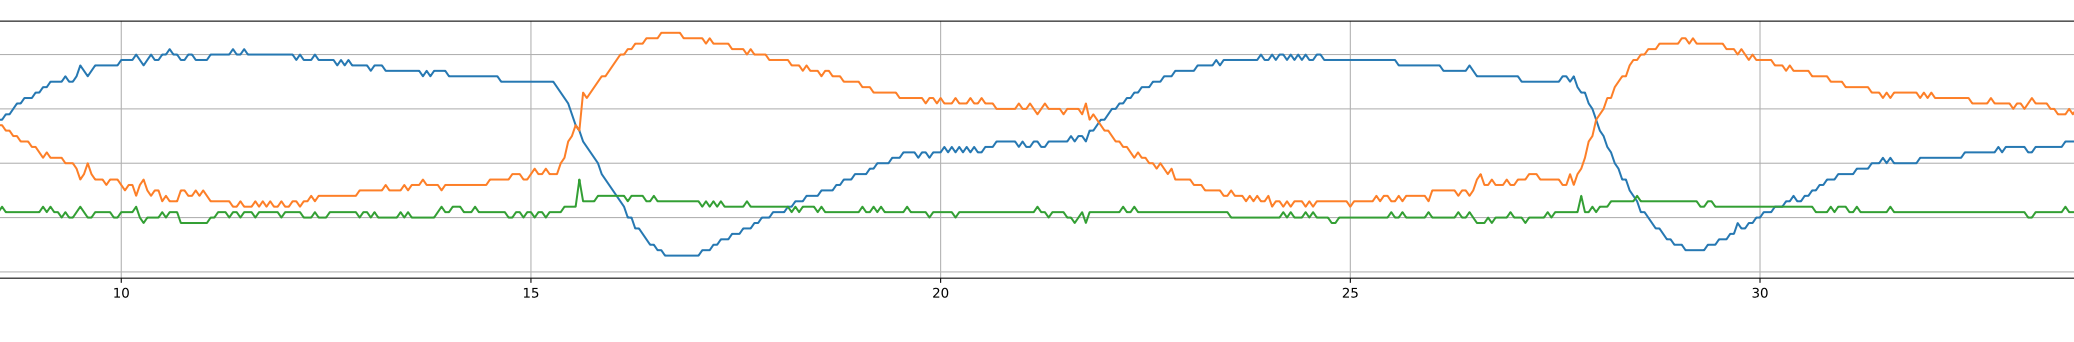
\includegraphics[width=0.6\paperwidth]{img/plots/battery.png}}
		\caption{Orientation affected by the battery charging.}
	\end{figure}
\end{center}

The current data flow is illustrated by the schema:

\begin{center}
	\begin{figure}[ht!]
		\makebox[\textwidth]{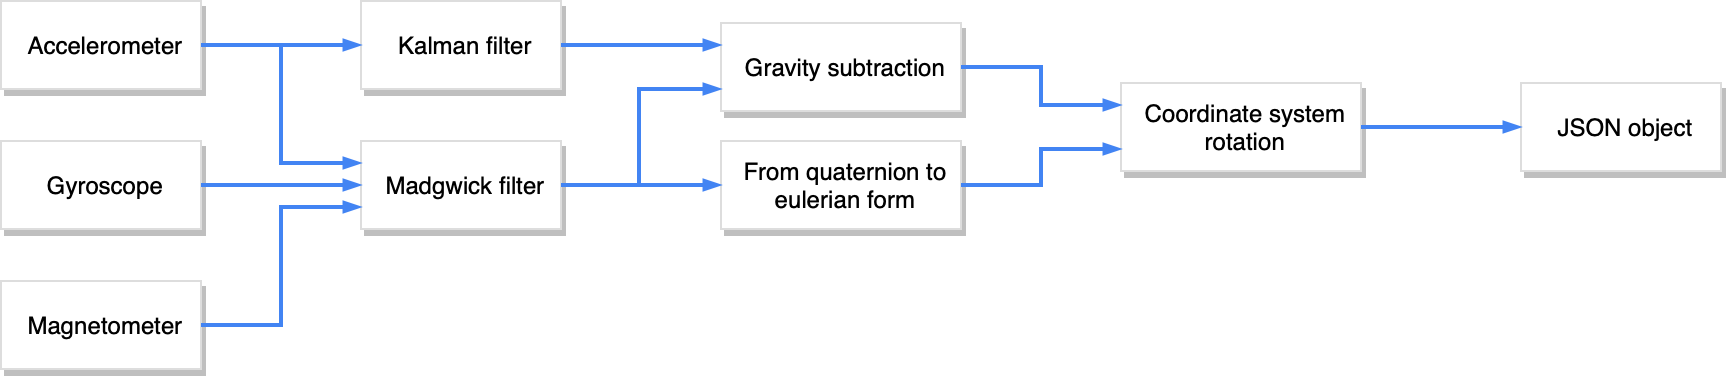
\includegraphics[width=0.65\paperwidth]{img/data_fusion.png}}
		\caption{Current data fusion schema.}
	\end{figure}
\end{center}

\section{Delay in real-time data plotting}
\dots
